Android is an open source \gls{os} launched in 2007 and today mainly maintained and developed by Google.
It is based on the Linux kernel and mainly targets touch screen devices such as mobile devices or wearables.
The system is designed to run efficiently on battery powered devices with limited hardware and computational capacity.
Android's main hardware platform is the ARM architecture, known for their low power consumption, but also runs on MIPS and x86 processors.
\newline
\newline
\begin{figure}[h]
    \centering
    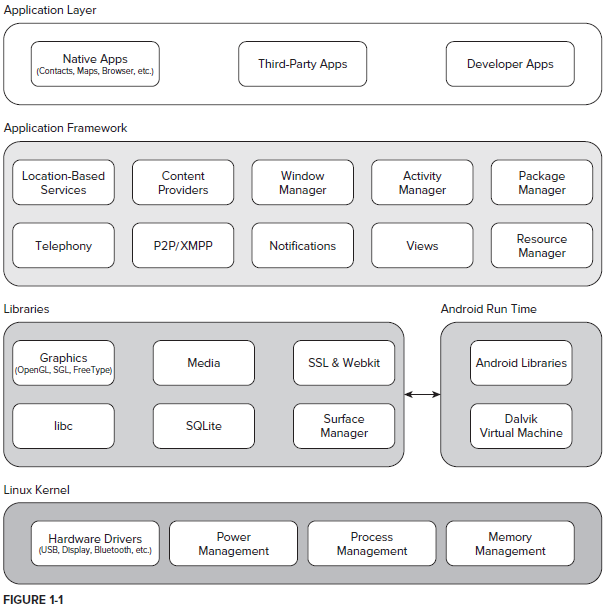
\includegraphics[width=0.8\textwidth]{data/stack.png}
    \caption{Android's architecture \cite{googleDalvik}}
    \label{fig:androidArchitecture}
\end{figure}
Figure~\ref{fig:androidArchitecture} gives an overview of Android's architecture.
\newline
The basis of the system is its kernel.
It is responsible for power and memory management and controls the device drivers.
\newline
The layer above the kernel contains the native libraries of the system and the Android Runtime.
\footnote[1]{While \gls{art} and \gls{dvm} are acronyms, they are also used to denote two different generations of runtime as will be described in section~\ref{subsection:android-dalvik} and in section~\ref{subsection:android-art}}
\newline
On top of the libraries and the runtime lies the application framework.
This layer provides generic functionality to applications over Android's \gls{api}, such as notification support.
\newline
The top layer is responsible for the installation and execution of applications.
\newline
This software allows Android to run on a wide range of devices with different hardware and offers a simple environment to run applications.
\newline
\newline
This chapter outlines the aspects of Android needed to understand the analysis and proposals.
